Anteriormente, en la imagen \ref{fig:docker-interface} se muestra cómo el
motor Docker interactúa con el kernel de Linux para proveer aislamiento. Entre
otras librerías, Docker usa en particular los \textit{cgroups} 
\autocite{Cgroups2021} y los \textit{namespaces} de Linux \autocite{LinuxNamespaces2021}.

Sendas funcionalidades del kernel ofrecen una gran capa de seguridad y aislamiento
de procesos de forma nativa en todas las máquinas Linux, y Docker aprovecha esa
infraestructura para proteger los contenedores a un nivel muy bajo: a nivel de
kernel.

Este planteamiento ya augura un buen presagio en tanto que no se usan aplicaciones
externas o librerías de terceros para el aislamiento y protección de capas sino
que se usa una arquitectura a bajo nivel ampliamente depurada y probada como es
el kernel de Linux. Además, esto permite también una gran portabilidad, ya que
el ``único requisito'' para ejecutar Docker sería contar con un kernel de 
Linux.

A la hora de hablar o revisar la seguridad de Docker, existen cuatro áreas
primordiales en las que indagar \autocite{DockerSecurity2021}:

\begin{itemize}
  \item La seguridad intrínseca del kernel así como su soporte para \textit{namespaces}
        y \textit{cgroups}.
  \item La superficie de ataque sobre el servicio de Docker en sí.
  \item Lagunas en las configuraciones de un contenedor o bien por defecto o bien
        introducidas por el usuario.
  \item Las características de seguridad del kernel y su interacción con Docker.
\end{itemize}

\subsubsection*{Linux kernel \textit{namespaces}}
A nivel de funcionamiento, Docker es similar a los contenedores LXC y comparten
los mismos mecanismos de seguridad. Por ende, cuando se crea un contenedor con el comando
\lstinline[style=bash]!docker run! internamente se están creando un conjunto
de \textit{namespaces} y \textit{cgroups} para el contenedor.

El primero ofrece la primera y mayor forma de aislamiento -- un proceso que se
ejecuta dentro de un \textit{namespace} es incapaz de ver (y mucho menos afectar)
a otros procesos en ejecución en otro contenedor o en la máquina anfitriona.

Esto llega al nivel de que cada contenedor tiene su propia pila de protocolos de
red, lo cual implica que un contenedor nunca tendrá acceso privilegiado a \textit{sockets}
o interfaces de otro contenedor o del sistema anfitrión. Sin embargo, si se configura
correctamente un sistema anfitrión las comunicaciones entre contenedores pueden
existir perfectamente, a través de la misma interfaz de red. Si por el contrario se
expone el puerto del contenedor entonces otros equipos podrán enviarle mensajes
o \textit{pings} al contenedor, paquetes TCP/UDP y establecer distintos tipos de
conexiones. Sin embargo, se pueden restringir si es necesario: a fin de cuentas,
la interfaz por defecto que usan los contenedores es la tipo puente, que implica
que en apariencia son equipos conectados a un \textit{switch}.

Por otra parte, los \textit{namespaces} de Linux tienen la ventaja de que son
prestaciones probadas y testeadas a lo largo del tiempo, introducidas en el año
2008 en la versión \texttt{2.6.15}. Además, su diseño y arquitectura
se basa en un intento de mejora sustancial de OpenVZ \autocite{OpenVZ2021},
desarrollado en 2005.

En un estudio realizado en el año 2018 \autocite{sunSecurityNamespaceMaking2018}, se
detectaron ciertos problemas residentes en el kernel que impedían a los contenedores
hacer uso de características avanzadas de seguridad del kernel: no se pueden
aplicar políticas para comprobar la integridad, regular la ejecución de código,
control de acceso, etc. que permiten prevenir problemas de seguridad referentes
a la aplicación. Ante el intento de añadir nuevas opciones al kernel que permitan
el acceso a dichos recursos, se descartaron debido a ser solución \textit{ad-hoc}
que suponían muchas veces una brecha de seguridad más allá de una opción
real.

Sin embargo, en dicho estudio se proponen los \textit{security namespaces}, una
característica del kernel que permitiría la ejecución de contenedores con la
totalidad de las prestaciones disponibles produciendo una latencia menor al
$0.7\%$ en las llamadas al sistema.

Esta característica ha seguido evolucionando hasta nuestros días en la forma de
los \textit{user namespaces}, que son los usados e implementados actualmente
por Docker. Un problema común del usuario \texttt{root} en Linux no es que sea
necesariamente el administrador sino las posibilidades que tiene (en particular,
las Linux kernel \textit{capabilites} \autocite{CapabilitiesLinuxManual}):
estas capacidades se pueden otorgar o bien mediante un escalador de privilegios
(por ejemplo, usar el comando \texttt{sudo}) o mediante el ajuste de permisos,
como el \texttt{SUID} o un cambio de \textit{namespace}. Esto se aprovecha por
el motor Docker para definir qué posibilidades tiene un contenedor, que pueden
ser añadidas o restringidas por el usuario.

El problema es cuando un usuario define un contenedor que requiere de más
capacidades de las que él mismo tiene. Por defecto, los contenedores se
ejecutan siempre como \texttt{root}, por lo que la situación anterior es
perfectamente posible, y conlleva posibles abusos en forma
de fallo de seguridad.

Con el uso de los \textit{user namespaces} este problema se puede abordar
fácilmente: un \textit{namespace} es a fin de cuentas un ``mapa'' en donde
un UID y GID virtuales se mapean con los UID/GID reales y se exponen
en la ruta \texttt{/proc} \autocite{blogEvolvingContainerSecurity2021}. El mapeo
presenta la siguiente forma (figura \ref{fig:ns-mapping}):

\begin{figure}[H]
  \centering
  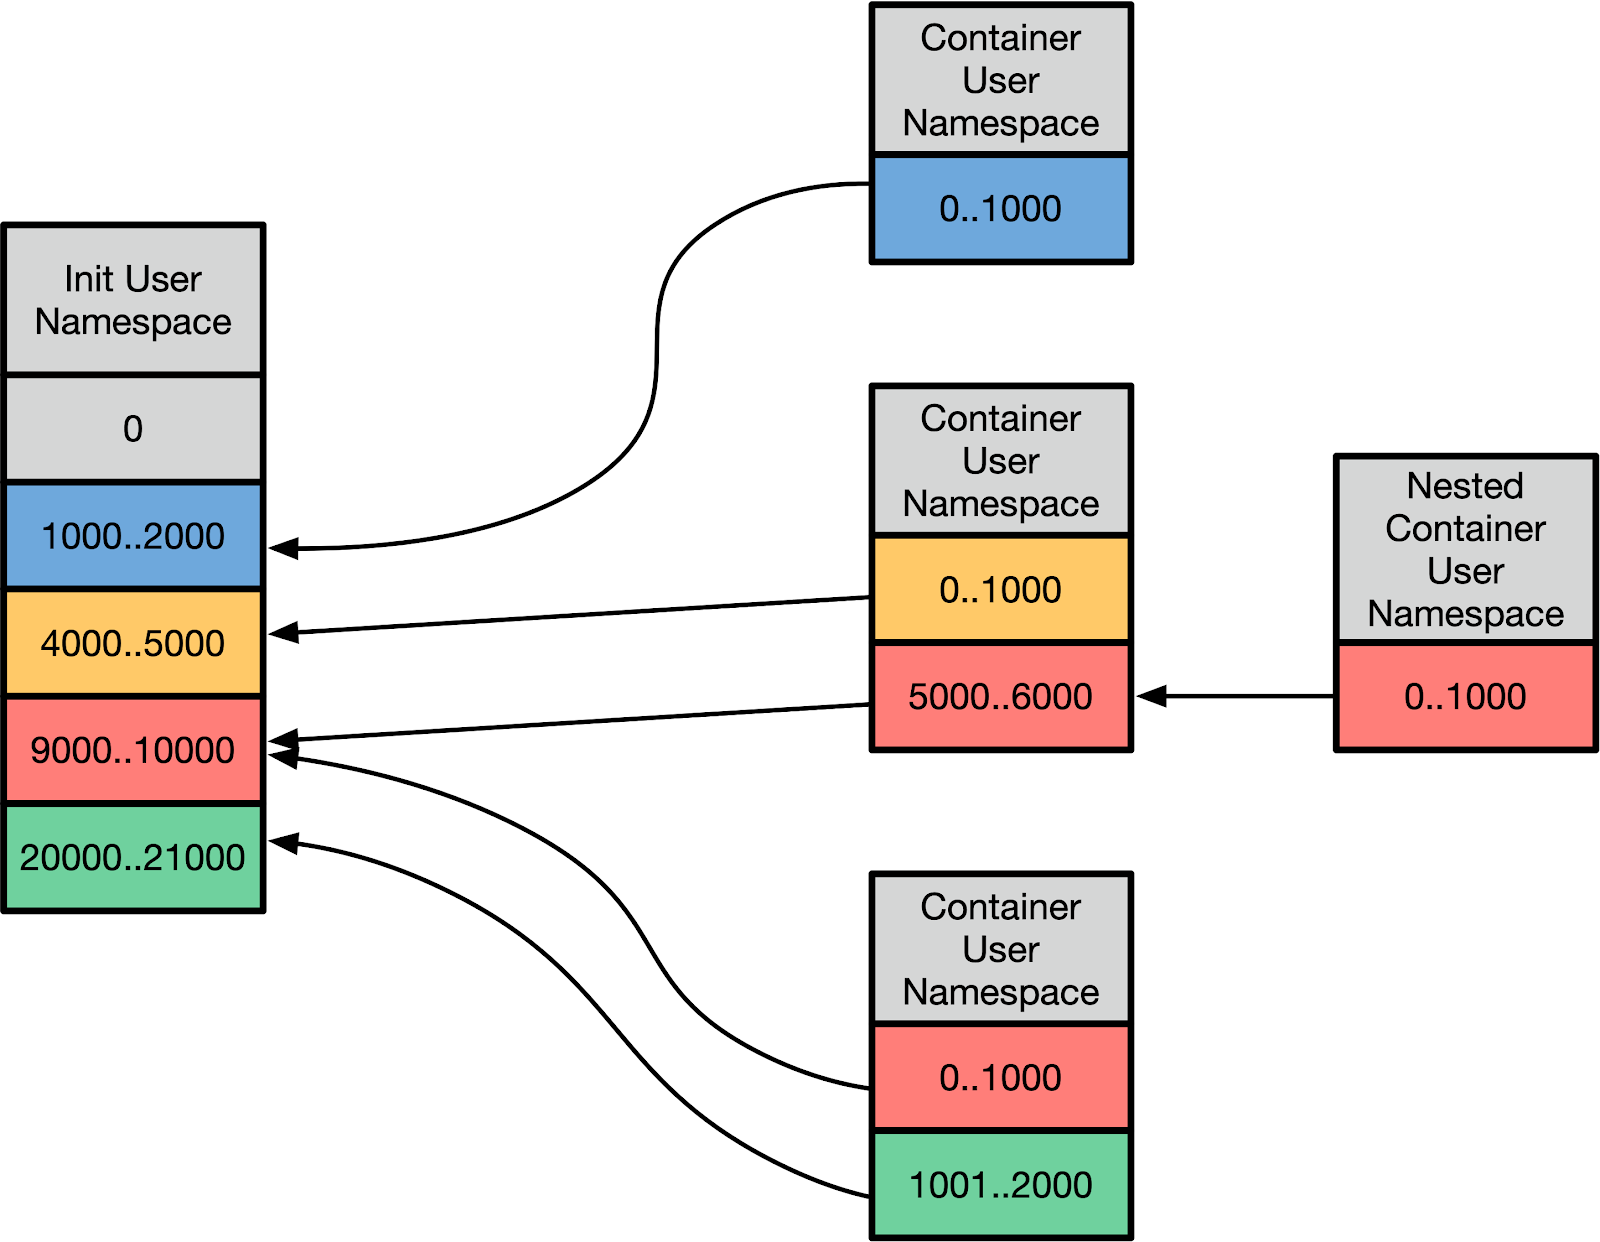
\includegraphics[width=\linewidth]{pictures/ns_mapping.png}
  \caption{Mapeo de los UID del \textit{namespace} del contenedor al \textit{namespace} del sistema \autocite{blogEvolvingContainerSecurity2021}.}
  \label{fig:ns-mapping}
\end{figure}

¿Por qué es potente esta característica del sistema?:

\begin{itemize}
  \item Permite, por una parte, definir ciertos UIDs únicamente dentro del
        contenedor. De esta forma, si un UID no está relacionado con un UID real
        del equipo anfitrión, al intentar examinar un fichero con dicho UID
        aparecerá un error del tipo \texttt{overflowuid} en los ficheros
        de \texttt{/proc} \autocite{DocumentationProcSys}.
  \item Desde el punto de vista de un \textit{namespace} de usuario el contenedor 
        se ejecuta con UID $0$ cuando en realidad está usando un rango de valores
        mapeados en dicho \textit{namespace}.
  \item Los subsistemas Linux pueden ejecutar la función \lstinline[style=C]!ns_capable!
        usando un \textit{namespace} específico de un recurso. De esta forma,
        los procesos pueden realizar acciones ``privilegiadas'' sin tener en
        realidad privilegios sobre el sistema anfitrión.
\end{itemize}

\subsubsection*{Linux \textit{control groups}
